\documentclass[tikz,border=2pt]{standalone}
\usepackage{amsmath}
\usetikzlibrary{arrows.meta}
\begin{document}
% FIFO single server, A = (1,2,5,9,10), S = (3,2,1,2,2), D = (4,6,7,11,13): a job's bar in the
% queue lane runs from A_k to the start of service, so its length is W_k; W = (0,2,1,0,1).
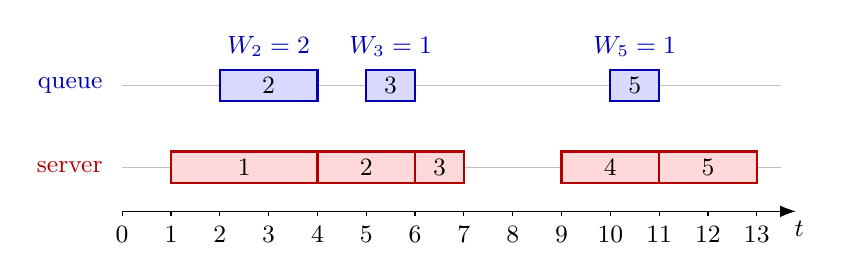
\begin{tikzpicture}[font=\small, >={Latex[length=2mm]}, x=0.62cm, y=0.8cm]
  % lane guides
  \draw[gray!50, thin] (0,1.3) -- (13.5,1.3);
  \draw[gray!50, thin] (0,0) -- (13.5,0);
  \node[anchor=east, blue!70!black] at (-0.2,1.3) {queue};
  \node[anchor=east, red!70!black] at (-0.2,0) {server};
  % waiting jobs
  \foreach \a/\b/\k/\w in {2/4/2/2, 5/6/3/1, 10/11/5/1} {
    \filldraw[blue!70!black, fill=blue!15, thick] (\a,1.05) rectangle (\b,1.55);
    \node at ({(\a+\b)/2},1.3) {$\k$};
    \node[blue!70!black, anchor=south] at ({(\a+\b)/2},1.6) {$W_{\k}=\w$};
  }
  % services
  \foreach \a/\b/\k in {1/4/1, 4/6/2, 6/7/3, 9/11/4, 11/13/5} {
    \filldraw[red!70!black, fill=red!15, thick] (\a,-0.25) rectangle (\b,0.25);
    \node at ({(\a+\b)/2},0) {$\k$};
  }
  % time axis
  \draw[->] (0,-0.7) -- (13.8,-0.7) node[anchor=north west, xshift=-4pt] {$t$};
  \foreach \t in {0,1,...,13} \draw (\t,-0.7) -- (\t,-0.78) node[below] {$\t$};
\end{tikzpicture}
\end{document}
